\documentclass[a4paper,12pt]{book}
%\usepackage[width=4.375in, height=7.0in, top=1.0in, papersize={5.5in,8.5in}]{geometry}

\usepackage{amsmath}
\usepackage{amssymb}
\usepackage{tipa}
\usepackage{eurosym}
\usepackage{graphicx}
\usepackage{fancyhdr}
\usepackage{xcolor}
\usepackage{ifpdf}
\usepackage{fullpage}
\ifpdf
\usepackage[protrusion=true,expansion=true]{microtype}
\usepackage{url}
\usepackage{hyperref}
\usepackage{breakurl}
\fi

\definecolor{hyperrefcite}{RGB}{0,51,153}
\definecolor{hyperrefurl}{RGB}{153,51,51}

\ifpdf
\hypersetup{
    bookmarks=true,
    unicode=false,
    pdftoolbar=true,
    pdfmenubar=true,
    pdffitwindow=false,
    pdfstartview={FitV},
    pdfpagelayout={SinglePage},
    pdftitle={Network Laboratory},
    pdfauthor={Ruizhi Liao, Alex Bikfalvi, Jaume Barcelo},
    pdfsubject={Practice},
    pdfcreator={LaTeX2e},
    pdfproducer={Universitat Pompeu Fabra},
    pdfkeywords={probabilities}{availability}{},
    pdfnewwindow=true,
    colorlinks=true,
    linkcolor=hyperrefcite,
    citecolor=hyperrefcite,
    filecolor=black,
    urlcolor=hyperrefurl
}
\fi

\pagestyle{fancy}
\renewcommand{\chaptermark}[1]{\markboth{#1}{}}
\renewcommand{\sectionmark}[1]{\markright{\thesection\ #1}}
\fancyhf{}
\fancyhead[LE,RO]{\bfseries\thepage}
\fancyhead[LO]{\bfseries\rightmark}
\fancyhead[RE]{\bfseries\leftmark}
\renewcommand{\headrulewidth}{0.5pt}
\renewcommand{\footrulewidth}{0pt}
\addtolength{\headheight}{0.5pt}
\setlength{\footskip}{0in}
\renewcommand{\footruleskip}{0pt}
\fancypagestyle{plain}{%
\fancyhead{}
\renewcommand{\headrulewidth}{0pt}
}

\parskip 0.05in

\begin{document}

\frontmatter
\pagestyle{empty}

\title{\textbf{Network Laboratory}}
\author{Ruizhi Liao, Alex Bikfalvi, Jaume Barcelo}
\maketitle

\tableofcontents

\mainmatter

\chapter{About the Course}

\section{Course Data}

Code: 21728

Course name: "Laboratori de Xarxes i Serveis"

Teachers: Ruizhi Liao, Alex Bikfalvi and Jaume Barcelo

Credits: 4

Year: 2nd year

Trimester: Spring

\section{Introduction}

The goal of this course is to acquire hands-on experience with networking equipment such as \emph{access points}, \emph{switches}, \emph{routers} and \emph{firewalls}. The students should be familiar with the high-level functionality of each of these devices. However, the actual configuration of the equipment and the construction of prototype networks will provide further insights into the operation of these network devices. After the course, the student will be ready to plan and configure a small network.

\section{Syllabus}
\begin{itemize}
  \item Lectures
  \begin{enumerate}
    \item Introduction to the Networking Laboratory
    \item Traffic analysis and IEEE 802.11 WLANs
    \item Virtual Local Area Networks and Spanning Tree Protocol
    \item Routers
    \item Firewalls
  \end{enumerate}
\item Lab Assignments
  \begin{enumerate}
    \item Traffic analysis
    \item IEEE 802.11 Wireless Local Area Networks (WLANs)
    \item Virtual local area networks (VLANs)
    \item Spanning Tree Protocol (STP)
    \item Routing
    \item Firewalls
  \end{enumerate}
\end{itemize}

\section{Bibliography}

TBD

\section{Evaluation Criteria}

The final grade is distributed as follows:
\begin{itemize}
\item Lab assignments, 70\%
\item Continuous assessment quiz, 10\%
\item Final exam, 20\%
\end{itemize}

The students need to obtain a passing mark (half of the available points) in all the different evaluation aspects.

\section{Group Work}

The assignments are done in groups of three students.
A single report is delivered for each group.
It is important that all the members of the group participate in the experiments and the preparation of the report.
The teachers may ask individual questions to the students in the labs, and the both the quiz and the final exam are performed individually.

\section{Lab Report}

For each lab assignment, it is necessary to prepare a lab report answering all the questions. The students are also expected to include additional information, explanation and comments besides those explicitly asked in the assignment.

\section{Survival guide}

\subsection{Questions and Doubts}

We like to receive questions and comments. Normally, the best moment to express a doubt is during the class, as it is likely that many people in the class share the same doubt. If you feel that you have a question that needs to be discussed privately, we can discuss it right after the class.

\subsection{Continuous Feedback}

At the end of lectures, we will ask you to provide some feedback on the course. In particular, we always want to know:
\begin{itemize}
\item What is the most interesting thing we have seen in class.
\item What is the most confusing thing in the class.
\item Any other comment you may want to add.

\end{itemize}

\subsection{How to Make Your Teachers Happy}

Avoid speaking while we are talking.

\chapter{Traffic Analysis}

\section{Introduction}

The goal of this lab assignment is to know and use monitoring and traffic analysis tools. We shall use the \emph{Wireshark} and \emph{tcpdump} software tools to study different layers of the TCP/IP architecture.

\section{Home Preparation}

Review the TCP/IP model and explain the function of each layer. Provide examples of the protocols at each layer of the protocol stack.

\emph{What is the purpose of ARP \cite{rfc826}}

Draw a sketch of the different messages being exchanged and the different steps involved.

\emph{Is it possible to run this protocol between computers that are in different local area networks (LANs)? What is the ICMP protocol?}

How does the \emph{ping} command work?
What does the \emph{ping} command measure?
Explain and draw an SSL connection indicating how the protocol works and which messages are being exchanged.

\section{Disable your local firewall}

On a Linux machine, your local firewall can interfere with the assignment.
Disable it using the command \texttt{service iptables stop} with root permissions.

\section{WireShark Network Analyzer}

Start your computer in Linux. Start the WireShark software program and choose the correct network interface from the \emph{Capture} $>$ \emph{Interfaces} dialog. Use it to start the packet capture. It is also possible to configure the length of the capture and other details.

\emph{What interface does WireShark detect? What is your IP address? What is the corresponding MAC address?}

Configure the \emph{Capture} $>$ \emph{Interfaces} options to perform a five minutes capture. Observe the results and answer the following questions.

\emph{What is the total number of captured packets? Are there lost packets? If yes, why?}

Select a (any) packet. Observe the details and answer the following questions.

\emph{What is the source and destination IP address? What are the source and destination MAC addresses? What is the number of bytes in the packet? What protocols can you see in the packet? Is there HTTP? If yes, what is the length of the HTTP message (the payload of the TCP segment or segments)? What are the source and destination port?}

In the dialog \emph{Analyze} $>$ \emph{Enable Protocols...}, it is possible to configure the protocols that WireShark will capture and display. Looking at the default protocols, find at least one protocol of each of the four upper layers of the TCP/IP stack (Application/Transport/Internet/Link). Include a brief description of the protocols you found.

Go to the menu \emph{Statistics} $>$ \emph{Protocol Hierarchy} and observe the percentage of the following protocols: Ethernet, Internet Protocol, TCP, UDP, Logical Link Control, ARP, STP, IPv6, HTTP.

\textbf{Include IPv6 practice with a ping to the local-link IPv6 address of a neighbor. Use: \texttt{ping6 -I iface addr} or a failed ping to \texttt{ping6 ipv6.google.com}.}

\emph{What are the differences between IPv4 and IPv6?}

\section{The ARP Protocol}

The Address Resolution Protocol (ARP) resolves the association between an IP address and a MAC address. It is used in IP over Ethernet networks. Capture traffic and analyze the ARP packets. You can filter the ARP packets writing "ARP" in the \emph{Filter Toolbar}.

\emph{What are the source and destination MAC addresses of the Ethernet frame that contains the ARP request message? Can you see the source and destination IP addresses in the ARP request frame?}

\textbf{Clear the ARP cache \texttt{sudo ip neighbour flush all}.}

Look for an ARP request-reply exchange and write the source and destination MAC and IP addresses.

\emph{What is the time elapsing between an ARP request and reply messages?}

Use the information available in WireShark to indicate the length of the ARP frames and draw the format of the messages.

\emph{To which layer does ARP belong?}

\section{HTTP and Secure HTTP}

Make a new 5 minutes capture and during this time visit a few web sites. After the capture is finished observe the different HTTP and HTTPS messages.
Use the filter toolbar to filter the messages. Observe an HTTP GET message and the corresponding response and answer the following questions.

\textbf{The filter for HTTP or HTTPS should be \texttt{http or ssl}.}

\emph{What is the HTTP version of your web browser? And the HTTP version of the server? What language does the client request to the server? Is it possible to find which are the URLs visited by the user? At which layer is this information available?}

The default destination port for web is 80 or 8080 when using a web proxy.

\emph{What is the source port of the get requests? Write the source port number for different connections. At which layer can you find this information?}

Find a DNS query/response pair.

\emph{What is the function of DNS?}

Use the option \emph{Analyze} $>$ \emph{Follow TCP Stream} to analyze a TCP session. Identify the three-way-handshake and the session tear-down.

\emph{If HTTP is used, it is possible to observe the contents of the web using WireShark?}

Now use HTTPS.

\emph{Is it still possible to read the information that is being transmitted?} Hint: look for SSL packets.

Identify a SSL handshake in WireShark.

\section{ICMP Ping Packet Capture (Homework)}

Close all the applications that use the network and ping four different web sites in four different continents. Analyze the results.

\emph{What protocols are used?}

Draw a frame and explain how the different packet are encapsulated in each other.

\emph{How many ping messages are transmitted by default?}

Prepare a table with the source, destination, and average packet delay  of the four different ping experiments.

\emph{What is the packet length? At which layers can we find source and destination addresses? Which kind of addresses? Are the ping packets sent uniformly in time? What about the answers? What are the reasons for different inter-arrival times for the answers? What information is included in the data field of the ICMP packets? What about in the reply messages?}

\section{tcpdump}

In this section we will use the \texttt{tcpdump} command in Linux. Use \texttt{man tcpdump} to learn about the different parameters and options of this command. With \texttt{tcpdump} it is also possible to filter the traffic according to the source or destination addresses, protocol, port number, etc.

Open a terminal and launch a \texttt{tcpdump} capture. Finish the capture using "Ctrl-C". What is the information provided by tcpdump and which format is being used? To which level does the information belong? Hint: remember that you can redirect the output using the command \texttt{\$ tcmpdump $>$ my-file}.

The first line of \texttt{tcpdump} specifies which interface is being used and it can be changed using the \texttt{-i} option. What interface are you using?

Describe the information provided for the ARP protocol (\texttt{tcpdump arp}).

Execute the same command again using the \texttt{-e} option. What is the difference with respect to the previous execution? Check the \texttt{tcpdump} manual if necessary.

Try several new captures related to this assignment, such as \texttt{tcpdump stp}, \texttt{tcpdump http}, \texttt{tcpdump http}, \texttt{tcpdump udp}, \texttt{tcpdump ssl}, \texttt{tcpdump ip}, etc. Try also to make captures for a specific IP address.

\chapter{LAN and WLAN}

\section{Home exercise}

Connect to the web configuration interface of your home access point and find:
\begin{itemize}
\item The name of the wireless network (SSID or ESSID).
\item Frequency channel.
\item PHY layer data rates.
\item Supported security protocols.
\item Possibility of QoS differentiation.
\end{itemize}

Do a survey and find the information of available wireless networks (name, channel, security settings).
You can use Netstumbler or the command ``sudo iwlist wlan1 scan''.

\section{Equipment}

Each group requires at least two PCs.
If possible, three PCs are better than two.
Boot one PC in Windows and the other one in Linux.
The hardware you are going to use is the Cisco Aironet 1200 access point.
The user guide can be downloaded here: \ifpdf \url{http://www.jaumebarcelo.info/teaching/lxs/wlan/WLAN_manual.pdf} \fi
The firmware of the access point is CISCO IOS Version 12.3(8)JA2.

Install an FTP server in one of the computers (e.g., \emph{Filezilla} in Windows or \emph{vsftpd} in Linux). You may use a web browser as an FTP client.

\begin{itemize}

\item[On Windows] Install and open Filezilla, and connect locally from the same PC using the loopback interface 127.0.0.1. Create a new user (username \texttt{test} and password \texttt{test}) and share a local folder with several large files. Do not forget to remove the proxy configuration, or select not to use a proxy server for local addresses.
    
\item[On Linux] Install \emph{vsftpd} with the command line \texttt{sudo yum install vsftpd}. Once installed, you can find and modify the FTP server configuration in the file \texttt{/etc/vsftpd/vsftpd.conf}. If you need to change the configuration, do not forget to restart the FTP server with the command \texttt{sudo services vsftpd restart}. The server allows by default anonymous access, and therefore you do not neet to create a new user. The default shared folder is \texttt{/var/ftp}.

\end{itemize}

\section{Disable your local firewall}

On a Linux machine, your local firewall can interfere with the assignment.
Disable it using the command \texttt{service iptables stop} with root permissions.

\section{Basic LAN Configuration}

Interconnect the windows box and the Linux box using a cross-over cable. --- ask Jaume
Check layer-2 connectivity using the LED or the \texttt{mii} command in Linux.
Check layer-3 connectivity and measure round-trip-time using ping.
Configure the interfaces if needed.
Estimate the available bandwidth using FTP transfer or iperf.
Change the speed to 10 Mbps (full duplex) and estimate the bandwidth again.

\emph{Is the maximum transmission speed reached? Why?}

\section{WLAN Basic Configuration}

WLANs can be used as an access point to LANs.
They can also be used to interconnect to LANs using WDS.

First connect the AP to the PC using Windows.
This can be either a direct connection or a connection using the patch panel.
You will find the AP's IP on a post-it, and the administrator user is \texttt{Cisco} and the password field is \texttt{Cisco}.

Use the express set-up to configure the AP.
AP Name: LABXARXES\_GRUP\_XX.
SSID: grupXX.
Channel: default.
Transmit power: default.

Make sure that the radio interface is up.
Indicate what are the security options available.
Try different settings and configurations and then connect the AP to the laboratory switch.

Connect the WiFi interface to the Linux box and connect the computer to the AP that you have just configured.
Disable the wired interface in order to make sure that you are using the wireless interface.
Check that you have network connectivity and use the \texttt{ifconfig} or \texttt{ipconfig} command to look at the interface configuration.

If you have network connectivity, you should be able to ping the other computers of your group (the ones with wired connection) and also be able to connect to the Internet.

Perform measurements from the wireless computer to the wired one and the other way around.
Measure the round-trip-time using ping.
Also the throughput using FTP to transfer a large file.
\emph{Can you reach the PHY rate maximum throughput? Why?}.
\emph{Do you observe the same values for the uplink and downlink?}
Write down any other observations you find interesting.

Use either ``Netstumbler'' or ``iwlist'' to detect the available wireless networks.
Write down their configuration.

Draw a sketch of the computers, access point and other networking devices in your setting.

\section{Hot-Standby}

The hot-standby is a feature to offer high availability.
A backup AP (AP-standby) takes over if the primary AP (AP-root) fails.

Collaborate with another group.
One of the groups will configure the AP-root and the other the AP-standby.
Make sure that you replicate the same configuration (with the exception of the IP address) in both devices.
Same SSID, same network mask and same security setting.

In the AP-root, go to ``Network Interfaces'', ''Radio 802.11g'', and select ''Access Point (Fallback to radio shutdown)''.

In the AP-standby select ``Services'', ``Hot Standby''.
Click enable and specify the MAC address that the AP will be monitoring (the radio interface of the root-AP).
If the configuration is correct, you should be able to see the status that will appear below on the screen.

Draw a sketch of all the involved network devices and connections and test that it actually works.
To test that it is working, disable the radio interface of AP-root (``Network interfaces'',``802.11g'',``settings'').
After the time-out expires, the AP-standby takes over with the same SSID and security settings.

To gather more information about what is going on, you can run ping tests while the takeover takes place.
You can also check the logs in the ``Home'' page of the AP configuration interface.
Finally, you can check the log of the Filezilla server.

\emph{How long does it take for the PC to recover the connection after AP-root's radio is disabled?
Will the user notice that the connection switches from one AP to the other? How?
Do you think that the default time-out setting are appropriate? Why?
How is the network affected if we change this parameters?
}

Now re-enable the radio interface of AP-root.
Then, at the AP-standby, click ``Restart''.
Check the information that appears in the ``Home'' page of the APs to determine to which AP is the client connected.

After you have verified that the client is connected to the AP-root device, disconnect the ethernet cable of AP-root.
\emph{What happens? Does the AP-standby take over? Why?}

\section{Configuring an AP as a Repeater}

A repeater AP is not connected to the wired LAN.
It is situated within the coverage range of another AP to extend the covered area.
Just in the previous exercise, both APs must share the same configuration (with the exception of the IP address).

In the AP-root, select the option ``role in radio network'' and then choose ``access point''.
In the AP-repeater (former AP-standby) disable the hot-standby option.
Configure the SSID and at the end of the page select ``Set Infrastructure SSID''.
In the ``express setup'' select ``Repeater'' in the option ``role in radio network''.

At this point, your home screen should show the configuration of your network and the repeater, and the clients connected to each AP.
Your client is probably connected to the AP-root.
Click on ``clients'' and you will see the list of associated clients.
You can de-associate a particular client if you select it.
The client will automatically re-connect to the repeater.

To verify that is working, repeat the round-trip-time and bandwidth tests that you have performed before.
Do the tests while connected on AP-root and AP-repeater.
\emph{Can you observe any difference?}
Repeat the ping tests while a file is being transferred.






\chapter{Virtual LANs (VLANs)}

In this lab assignment the switches will be configured to create different VLANs.
The IPs of the switches are 192.168.1.110, 192.168.1.111 and 192.168.1.112.
An sketch on the blackboard specifies the switch to which your PC is connected.
Each VLAN has a unique identifier that takes values between 0 and 4094. 
In this assignment we will use the identifiers 10 and 20.


Each group will use three PCs.
One of the PCs is for managing the switch and needs an IP address of the same range as the IP of the switch (check the blackboard for the details).
The IPs of the other two switches must belong to the range of the VLAN that you are going to use (192.168.\{10,20\}.XX).

\section{Creation of a VLAN}

\begin{table}[!t]
%% increase table row spacing, adjust to taste
\renewcommand{\arraystretch}{1.3}
% if using array.sty, it might be a good idea to tweak the value of
%\extrarowheight as needed to properly center the text within the cells
\caption{Command modes}
\label{tab:modes}
\centering
\begin{tabular}{|c|p{5cm}|c|}
\hline
Command Mode & Access & Prompt\\
\hline
User EXEC & Connecting to the switch & Switch> \\
Privileged EXEC & Using the enable command in the ``User EXEC'' mode & Switch\# \\
Global Configuration & Using the ``configure terminal'' command in the ``Privileged EXEC'' mode& Switch(config)\# \\
        Interface Configuration & Using the ``interface $<$interface-name$>$'' command in the ``Global Configuration'' mode specifying the interface that we want to configure, e.g. FastEthernet0/4& Switch(config-if)\# \\
\hline
\end{tabular}
\end{table}


Table \ref{tab:modes} describes the four possible modes of interaction with the switch.
The first one offers limited information about the switch.
It is possible to find more detailed information in the second (privileged EXEC) mode.
The third mode allows the configuration of general aspects of the switch while and the last one is to configure a specific interface.
The commands available in each of the modes are different.
Make sure you are in the right mode before issuing a command.
It is possible to move to the previous mode using the ``exit'' command.

Use a telnet client to connect to the switch and observe which is the initial mode.
You can use the command ``?'' to obtain information about the possible commands in a given mode.
Additionally, you can also follow a partial command by ``?'' to obtain more information about how to use the command and the required parameters.
For example ``ip address ?'' would give you information about the parameters you could use after address.

Enter the mode \emph{privileged} EXEC and use the command \texttt{show running config} to see the current configuration of the switch.
Answer the following questions.
\emph{How many VLANs can you observe? (Note that this is not necessarily the number of VLANs in the switch).}
\emph{How many Fast Ethernet interfaces are available?}
\emph{What is the VLAN1 administrative address?}
\emph{What is the status of VLAN1?}

There exists a \emph{default} VLAN which has the number 1.
Use the command \texttt{show vlan}.
\emph{How many VLANs are there in the switch?}
For each of the interfaces identify the ID, the name, the status, the assigned ports and the type.
Include this information in the report.

Enter the config mode and try to delete the default VLAN: 
\texttt{Switch-B(config)#no vlan 1}.
\emph{What happens?}

In the config mode, use the ``?'' to find which commands can be used in this mode.
Use the \texttt{vlan <id>} to create a new command.















\chapter{Spanning Tree Protocol (STP)}

\section{Switch Manual}
The user manual for the switch is available here:

\url{http://www.jaumebarcelo.info/teaching/lxs/stp/manual_spantree.pdf}

\section{Introduction}

In this assignment you will configure the Spanning Tree Protocol (STP). This protocol is used in Ethernet networks to establish which are the active link and therefore which is the path that data packets will follow. The switches that you will use are the same as the ones in the previous assignment. Have your VLAN report handy just in case you need to consult it and to remember which are the basic commands to interact with the switch.

\section{Theoretical Construction of the Tree}

The switches are connected as illustrated in the figure \ref{fig:StpTopology}.

\begin{figure}
\centering
\ifpdf
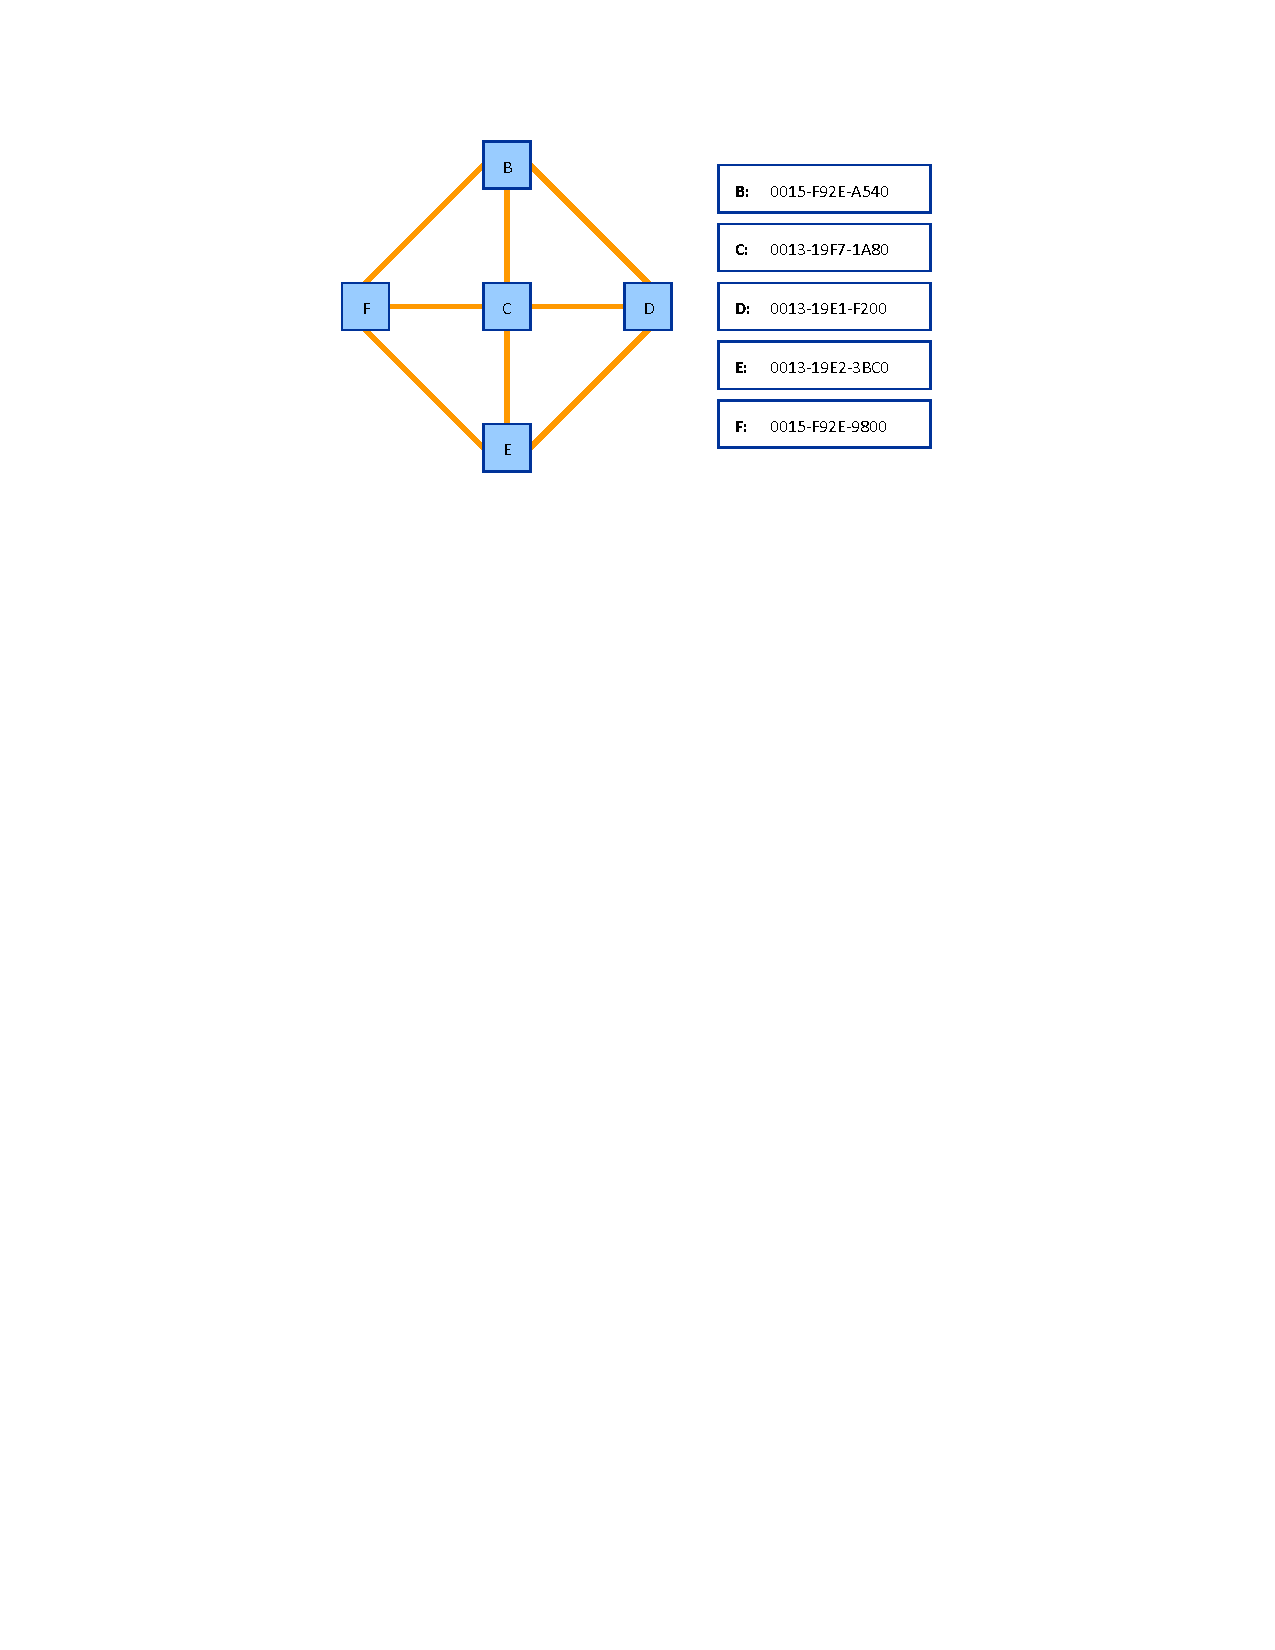
\includegraphics[width=0.9\linewidth]{Figures/StpTopology.pdf}
\else
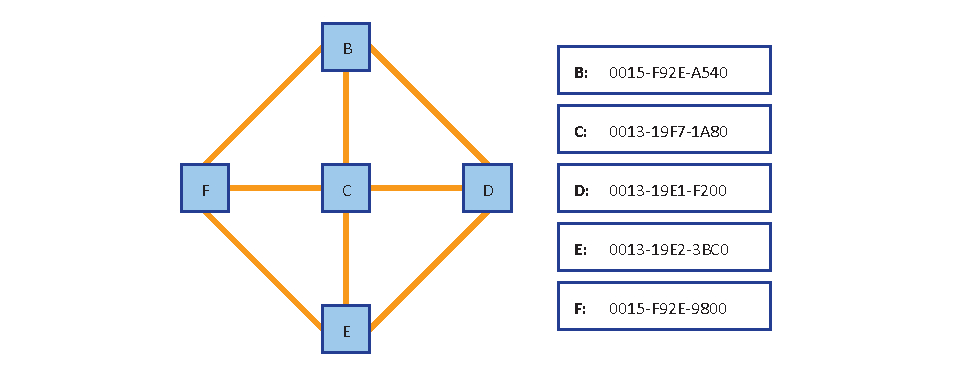
\includegraphics[width=0.9\linewidth]{Figures/StpTopology.eps}
\fi
\caption{The network topology used for the STP practical exercise.}
\label{fig:StpTopology}
\end{figure}

\begin{center}
\sffamily\small
\begin{tabular}{>{\columncolor{tablegray}}p{15cm}}

\multicolumn{1}{>{\columncolor{tableorange}}l}{Questions and Tasks}\\
Find the \texttt{\color{blue}BridgeId} of each switch.\\
\hline
Compute which is the spanning tree and draw it.\\
\hline
Which is the root switch?\\
\hline
Which is the role of each port?\\
\hline
Which are the activated ports?\\
\hline
\end{tabular}
\end{center}

Fill in the table \ref{tab:Stp}.


\begin{table}
\sffamily\small
\centering
\begin{tabular}{>{\columncolor{tablegray}}ccccc}
\multicolumn{1}{>{\columncolor{tableorange}}c}{Switch ID} & \multicolumn{1}{>{\columncolor{tableheader}}c}{MAC} & \multicolumn{1}{>{\columncolor{tableheader}}c}{Port} & \multicolumn{1}{>{\columncolor{tableheader}}c}{Role} &
\multicolumn{1}{>{\columncolor{tableheader}}c}{State} \\
Switch B & & & & \\
\cline{2-5}
& & & & \\
\cline{2-5}
& & & & \\
\hline
\vdots & & & & \\
\hline
\end{tabular}
\caption{The spanning tree.}
\label{tab:Stp}
\end{table}

\section{Practical Verification}

Now you will verify that the STP constructed by the switches is in fact the one you computed in the previous section. Use the VLAN 1 to connect to the five switches (B, C, D, E, F). It is recommended to open five simultaneous Telnet connections, one for each of the switch.

Each group will work in a different VLAN. The teacher will assign a VLAN to each group. Make sure that your VLAN is included in all the trunk ports. Each group will have a different STP, as the network creates a tree for each VLAN.

In each of the switches, enter the \emph{privileged EXEC} mode and use the command:

\begin{lstlisting}
Switch# show spanning-tree vlan <id>
\end{lstlisting}

\begin{center}
\sffamily\small
\begin{tabular}{>{\columncolor{tablegray}}p{15cm}}

\multicolumn{1}{>{\columncolor{tableorange}}l}{Question}\\
What can you see?\\
\hline
\end{tabular}
\end{center}

Observe all the fields and make sure you understand them.

{\color{red}Find the BridgeId of each switch.
Compute which is the spanning tree and draw it.
Which switch is the root?
Which is the role of each port?
Which ports are activated?

Fill in the table \ref{tab:Stp} and compare practical results to the theoretical computation.}

\section{Changing the STP Configuration}

Now that you are familiar with the STP parameters, you will make some changes that will result in the computation of a new tree. In the \emph{global configuration} mode use the command:

\begin{lstlisting}
Switch(config)# spanning-tree vlan <id>
\end{lstlisting}
or, alternatively, you may use:

\begin{lstlisting}
Switch(config)# interface vlan <id>
Switch(config)# spanning-tree
\end{lstlisting}
to see which parameters are susceptible to be configured. Use the question mark \texttt{\color{blue}?} to see all the available parameters and make sure you understand them.

The exercise that we propose is to change the priority of one of the switches different from the root switch. The default behavior is that the switch with the lowest MAC address is selected as a root. The reason is that, in the default configuration, the priority of all the switches is 32768. By changing the priority of one of the switches to a lower value, we can force that that particular switch becomes the root.

Go ahead and change the root switch and observe the new configuration of the tree. Fill in the table \ref{tab:Stp} for this new configuration and draw the new tree.

\section{Link Failure}

This exercise cannot be started until all the groups have finished the previous one. If you reach this exercise before the other groups, move on to the next exercise while you wait for all the groups to be ready for the link failure.

Now we will disconnect one of the links to simulate a link failure. Compute in advance your new spanning tree after the link failure. Ask your teacher which is the cable that will be disconnected.

After the disconnection, check which is the new configuration and compare it with the one that you have predicted. Explain what happened.

\section{BPDUs}

Use the computer connected to the VLAN 1 (the computer used for the administration of the switch) and capture the traffic for several seconds using \emph{Wireshark}. Observed the received STP frames and identify the different fields in the packet. Write them down to include them in your report and find out which is the meaning of the information in each of the fields.

\begin{center}
\sffamily\small
\begin{tabular}{>{\columncolor{tablegray}}p{15cm}}

\multicolumn{1}{>{\columncolor{tableorange}}l}{Question}\\
Why are you receiving these frames at your computer?\\
\hline
\end{tabular}
\end{center}


\backmatter
\bibliographystyle{plain}
\bibliography{rfc,my_bib}
\end{document}
\end{document}
